\chapter{Petalinux - Creating tailor-made OS for FPGAs SoMs}
Petalinux is an embedded Software Development Kit - SDK - targeting FPGA-based System on a Chip - SoC - design or FPGA designs.

\subsection{Setting up the environment}
Before the actual installation of petalinux, some setting of the environment is needed.
There are few steps to be followed in order to make the environment work:
\begin{itemize}
	\item Adding the 32-bit architecture to the system
	\item Installing the TFTP server (if needed)
	\item Installing all the required packages for the petalinux Build Host 
\end{itemize}
The first step is taken care of by typing
\begin{verbatim}
	sudo dpkg --add-architecture i386
\end{verbatim}
followed by
\begin{verbatim}
	sudo apt-get update
\end{verbatim}
This two commands will add the 32-bit architecture and update apt-get, so as to make the changes effective. To see if the architecture has been properly added, type
\begin{verbatim}
	dpkg --print-foreign-architectures
\end{verbatim}
and an output like the one of Fig \ref{fig:i386added} will be shown.
\begin{figure}[ht]
	\centering
	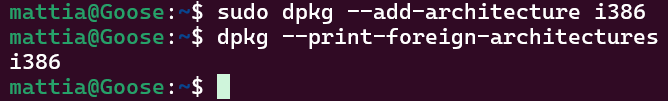
\includegraphics[width=0.65\textwidth]{images/i386added}
	\caption{Successful installation of i386 architecture.}
	\label{fig:i386added}
\end{figure}

The installation of the TFTP server is done by following the subsequent commands.
\begin{verbatim}
	sudo apt-get upgrade
	sudo apt-get update
\end{verbatim}
and a window similar to that of Figure \ref{fig:tftp1} will appear.
\begin{figure}[ht]
	\centering
	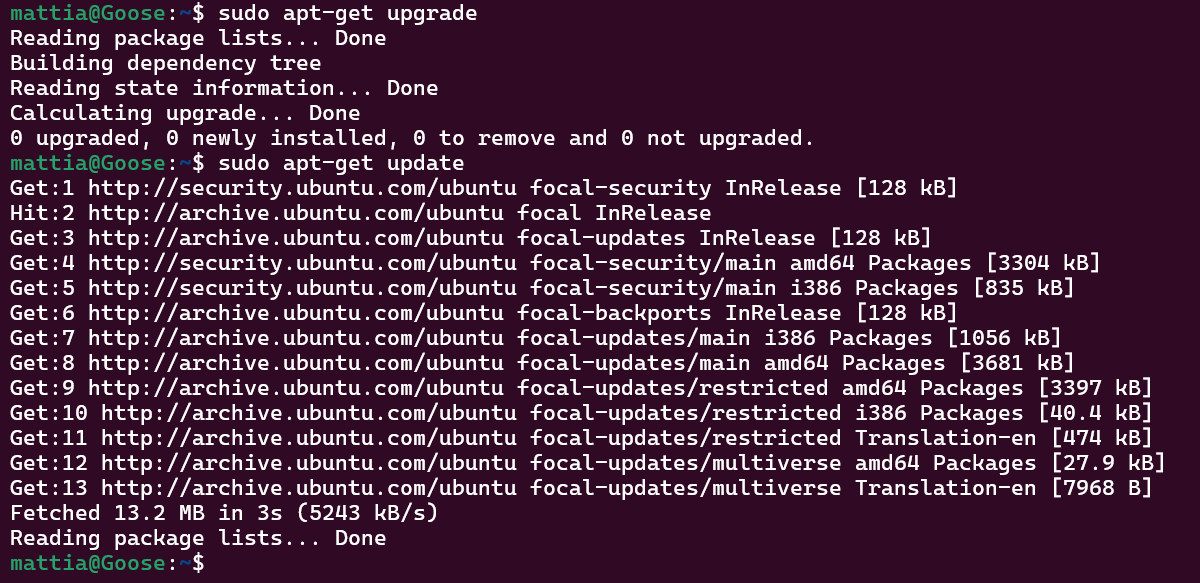
\includegraphics[width=0.65\textwidth]{images/tftp1}
	\caption{Apt upgrading and updating.}
	\label{fig:tftp1}
\end{figure}
Now it is possible to actually install the TFTP server. Type
\begin{verbatim}
	sudo apt-get install tftpd-hpa
\end{verbatim}
and let the computer run the respective task. Once it is done, check for the correct installation typing
\begin{verbatim}
	sudo systemctl status tftpd-hpa.service
\end{verbatim}
and the output of Figure \ref{fig:tftp3} should appear. To start the server automatically during the boot, type
\begin{verbatim}
	sudo systemctl enable tftpd-hpa
\end{verbatim}
\begin{figure}[ht]
	\centering
	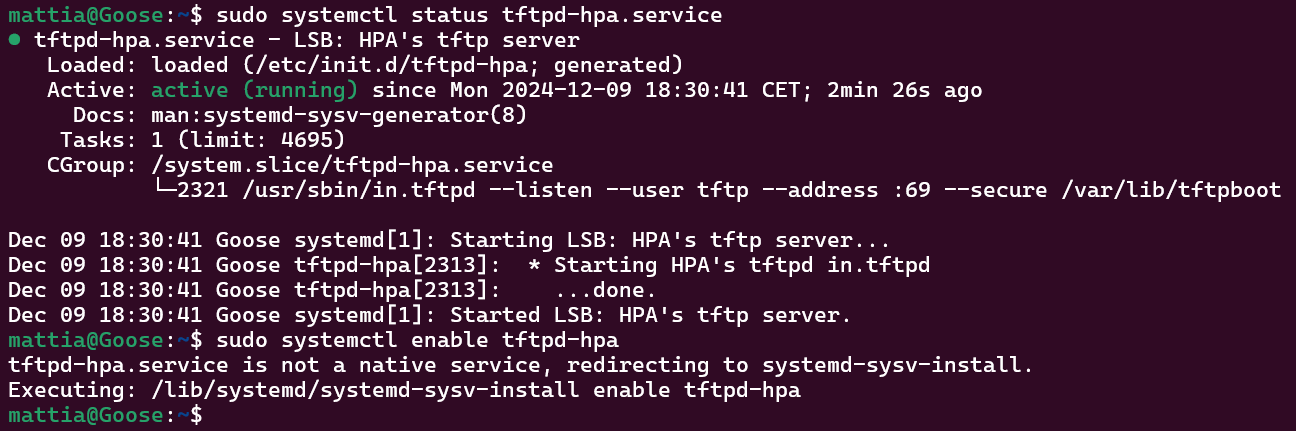
\includegraphics[width=0.65\textwidth]{images/tftp3}
	\caption{Correctly running TFTP server.}
	\label{fig:tftp3}
\end{figure}
Now the server should be all set. After the installation, it is necessary to configure the server. Type
\begin{verbatim}
	sudo nano /etc/default/tftpd-hpa
\end{verbatim}
and in the window that will open write down the following text
\begin{verbatim}
	TFTP_USERNAME="tftp"
	TFTP_DIRECTORY="/var/lib/tftpboot"
	TFTP_ADDRESS="0.0.0.0:69"
	TFTP_OPTIONS="--secure"
\end{verbatim}
as shown in Figure \ref{fig:tftpconf}.
\begin{figure}[ht]
	\centering
	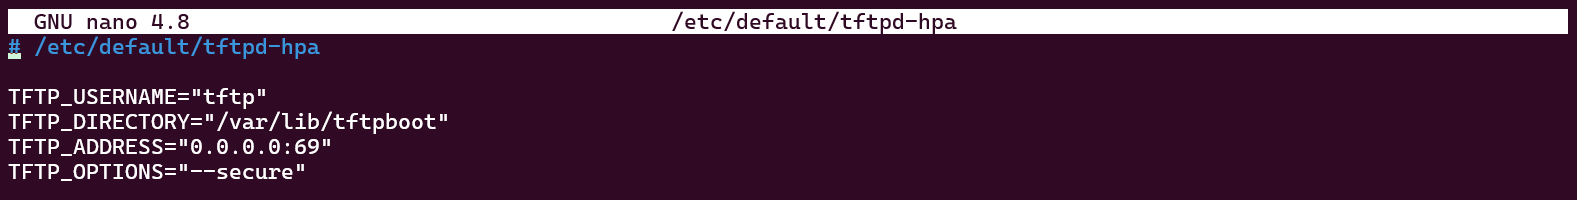
\includegraphics[width=0.65\textwidth]{images/tftpconf}
	\caption{Setting TFTP server.}
	\label{fig:tftpconf}
\end{figure}
Then, finish the configuration with the following commands (one per time)
\begin{verbatim}
	sudo mkdir -p /var/lib/tftpboot
	sudo chown -R nobody:nogroup /var/lib/tftpboot
	sudo chmod -R 777 /var/lib/tftpboot
	sudo systemctl restart tftpd-hpa
\end{verbatim}

A trick that will come in hand is to link the Windows downloads folder and the Vivado workspace with a custom-made folder within the WSL. To do so type the following command in the WSL shell (on the same line)
\begin{verbatim}
	sudo ln -s /mnt/c/Users/<folder_path>/<folder_name> ~/<new_folder_name>
\end{verbatim}
The results will be the one shown in Figure \ref{fig:symlink}
\begin{figure}[ht]
	\centering
	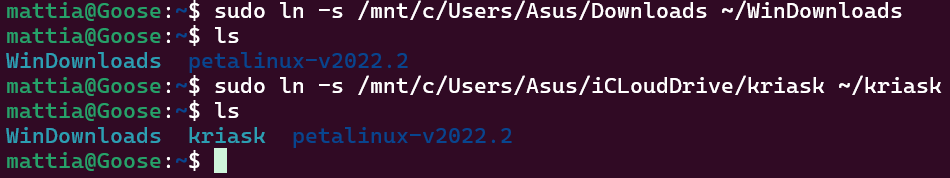
\includegraphics[width=0.65\textwidth]{images/symlink}
	\caption{Successful link created.}
	\label{fig:symlink}
\end{figure}

Finally, all the needed packages can be installed. From this \href{https://adaptivesupport.amd.com/s/article/73296?language=en_US}{page}, download the file at the bottom. Create the folder in which petalinux will be installed with the command
\begin{verbatim}
	mkdir <folder_name>
\end{verbatim}
In this tutorial it is named \textit{petalinux-v2022.2} (see Figure \ref{fig:symlink}). Copy the file from the download folder to the bespoke petalinux installation folder by typing
\begin{verbatim}
	cp <start_path> <final_path>
\end{verbatim}
and then type
\begin{verbatim}
	chmod +x <installer_file_name>
	sudo ./<file_name>
\end{verbatim}
Once the installation is complete, all the packages should have been installed. it might be necessary to reinstall the tftpd-hpa server after this operation.


Now it is possible to begin the actual installation of petalinux. From the petalinux \href{https://www.xilinx.com/support/download/index.html/content/xilinx/en/downloadNav/embedded-design-tools/archive.html}{AMD download page}, download the needed version and move it to the installation folder. From this page also download the .BPS file relative to the board to be used. This latter file has to be moved into the folder in which the petalinux project are saved. Now type
\begin{verbatim}
	chmod +x <installer_file_name>
	./<file_name>
\end{verbatim}
if an error message appears (Fig. \ref{fig:error_log}), then type
\begin{verbatim}
	sudo chmod 666 petalinux_installation_log
	./<installer_file_name>
\end{verbatim}
Now the installation should begin. By following the instruction, the installation process should proceed without any inconvenience, even though it might take a while. 
\begin{figure}[ht]
	\centering
	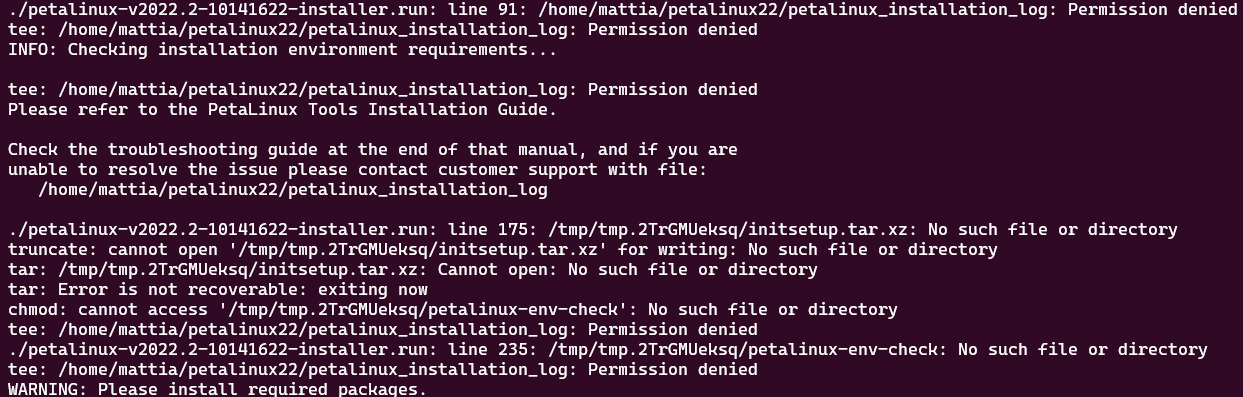
\includegraphics[width=0.65\textwidth]{images/error_log}
	\caption{Output error.}
	\label{fig:error_log}
\end{figure}
Finally, to set the petalinux environment into the directory in which it is installed, type
\begin{verbatim}
	source settings.sh
\end{verbatim}
from which the shell output highlighted in Fig. \ref{fig:envset} is shown.
\begin{figure}[ht]
	\centering
	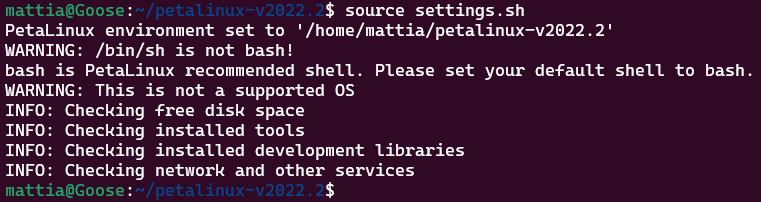
\includegraphics[width=0.65\textwidth]{images/envset}
	\caption{Setting petalinux environment.}
	\label{fig:envset}
\end{figure}
Now the system should be all set. The [WARNING] message relative to the OS system is due to the used version of Ubuntu, that is Ubuntu 20.04.6, which is not among the supported OS listed by AMD.

Due to the high load that the following process will constitute for a normal device, the guide from now on will refer to a server running CentOS Stream 9. All the procedure, however, should be the same, except minor errors or problems.
